\section{SoftEther}
\subsection{Overview}
SoftEther è una tecnologia per VPN molto particolare, sviluppata da uno studente
giapponese per la sua tesi di laurea magistrale (ora è diventato \textit{associate professor}),
è un progetto
attivamente sviluppato, open source e gratuito.\\
E' disponibile cross-platform, Linux, MAC OS X e Windows. Per
le versioni MAC OS X e Windows è disponibile un'interfaccia grafica sia per client
sia per server, che consente di configurazioni in maniera molto intuitiva; su Linux
bisogna cavarsela con file di configurazione ed una shell (\texttt{vpncmd}).


La particolarità di questo software è che in grado di gestire anche \textit{altri}
protocolli VPN, oltre a quello sviluppato appositamente per SoftEther.
I protocolli supportati sono:
\begin{itemize}
  \item SoftEther (VPN over HTTPS);
  \item OpenVPN (L2  e L3);
  \item SSTP (PPTP over TLS);
  \item L2TP/IPsec;
  \item L2TPv3/IPsec;
  \item EtherIP.
\end{itemize}
Il grande vantaggio che dà l'utilizzo del protocollo SoftEther è l'incapsulamento in
HTTPS, per cui si usa tutta la sicurezza derivante da TLS, unitamente al fatto che
praticamente qualsiasi firewall lascerà passare questo traffico.\\
La figura \ref{fig:softether-archi} mostra come funziona SoftEther.


SoftEther è composto da diversi software:
% \begin{figuare}
%   \includegraphics{img/sofether_scheme}
%   \caption{}
% \end{figuare}
\begin{itemize}
  \item \textit{VPN Server}: il componente server in grado di gestire i multipli
  protocolli VPN.
  \item \textit{Virtual Hub}: a dispetto del nome è uno switch che viene usato internamente
  dal VPN Server per collegare i diversi tunnel.
  \item \textit{Virtual L3 Switch}: anche in questo caso il nome trae in inganno, poiché si tratta di un
  router che si utilizza in topologie LAN-to-LAN.
  \item \textit{Local Bridge}: componente del server che viene usato per collegare la rete dei Virtual Hub
  alla rete fisica su cui si trova il server VPN. E' necessario avere un'interfaccia di rete
  fisica dedicata che sia connessa ad uno switch (su cui non sia attivo nessun protocollo di rete);
  è possibile anche utilizzare una scheda di rete virtuale usando \texttt{TAP} al layer 2.
  E' comunque consigliabile
  una NIC di buona qualità, che possa lavorare in modalità promiscua. Non è obbligatorio
  avere questa seconda interfaccia, sebbene sia caldamente consigliato.
  \item \textit{VPN Bridge} è la combinazione di \textit{Virtual Hub} e \textit{Local Bridge} che consente
  di collegare tra loro diverse \textit{reti} in VPN (e non singoli host). E' utilizzabile
  lato client per realizzare topologie LAN-to-LAN.
  \item \textit{VPN Client} è il classico componente client che connette un PC ad una VPN. Utilizza il
  protocollo SoftEther VPN sopra descritto. Come client si può comunque utilizzare un qualsiasi software che
  usi uno dei protocolli sopra citati. E' da utilizzare solo in configurazioni Remote Access.
\end{itemize}


\begin{figure}
  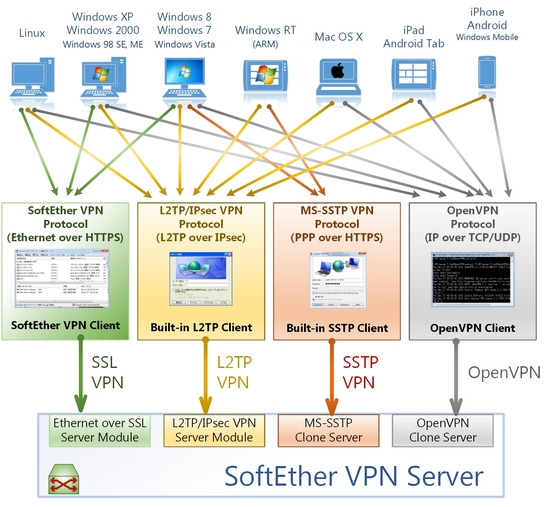
\includegraphics[scale=0.45]{img/softether_scheme}
  \label{fig:softether-archi}
  \caption[Il design di SoftEther]{Il design di SoftEther. Mediante il \textit{Virtual Hub} si \textit{collegano} i diversi
  moduli.}
\end{figure}
Con SoftEther si possono realizzare le topologie:
\begin{itemize}
  \item \textbf{Remote Access}. Si crea in maniera molto semplice una nuovo server, mediante la GUI o
  la linea di comando. Dal punto di vista logico si fanno i seguenti passaggi:
  \begin{enumerate}
    \item creazione di un nuovo server;
    \item creazione di un nuovo \textit{Virtual Hub} che ``riceve le connessioni'';
    \item connessione del \textit{Virtual Hub} alla scheda di rete del server (possibilmente dedicata a fare
    questo). Così facendo si dà accesso alla rete in cui si trova il server.
    \item Connessione al server utilizzando il software client.
    \begin{figure}
      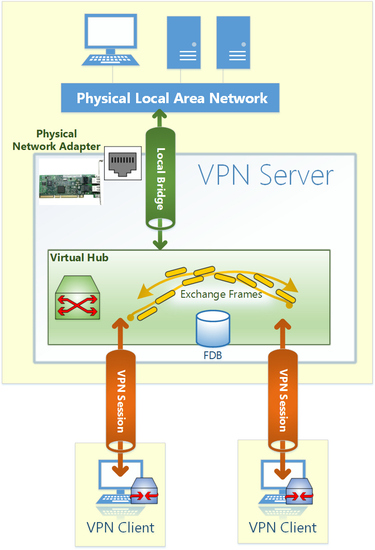
\includegraphics[scale=0.4]{img/softether_ras}
      \label{fig:softether_ras}
      \caption[Configurazione di SoftEther per Remote Access VPN]{Configurazione di SoftEther per Remote Access VPN.}
    \end{figure}
  \end{enumerate}
  \item \textbf{LAN-to-LAN}. E' possibile scegliere se collegare le diverse (non necessariamente 2) LAN
  a livello 2 o a livello 3, le differenze tra le due sono già state descritte
  in precedenza.
  Una volta scelta la topologia che si preferisce si crea un \textit{VPN server}, poi occorre
  differenziare in base al livello.
  \begin{itemize}
    \item L2:
    \begin{enumerate}
      \item sulla rete da connettere al server si crea un nuovo \textit{VPN Bridge};
      \item si connette il bridge al server (si chiama \textit{cascaded connection});
      \item si connette il bridge alla LAN locale utilizzando \textit{Local Bridge}.
      \begin{figure}
        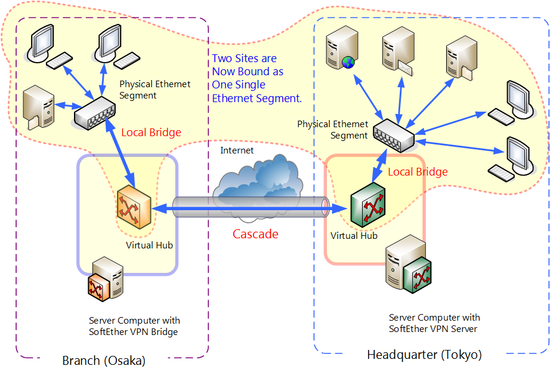
\includegraphics[scale=0.55]{img/softether_l2_lan_to_lan}
        \label{fig:softether_l2_lan_to_lan}
        \caption[Configurazione LAN-to-LAN con SoftEther al layer 2]{Configurazione LAN-to-LAN con SoftEther al layer 2.}
      \end{figure}
    \end{enumerate}
    \item L3:
    \begin{enumerate}
      \item sul server si creano $n$ \textit{Virtual Hub}, uno per ogni LAN remota che si vuole
      collegare; esso ``accumula'' tutte le connessioni provenienti da ciascuna LAN;
      \item si configura uno \textit{Virtual L3 Switch} che connette i 3 hubs. A dispetto del nome,
      esso si comporta come un router, per cui avrà $n$ interfacce di rete, ciascuna di esse con un
      indirizzo IP compatibile con quello della LAN remota. Per cui l'interrfaccia connessa al \textit{Virtual Hub 1}
      dovrà avere un IP che sia compatibile con gli indirizzi IP della LAN che si ``accumula'' nel \textit{Virtual
      Hub 1}.
      \item Per ciò che concerne i client, si utilizza un \textit{VPN Bridge} come
      per L2.
      \item L'ultimo step prevede di configurare, su ciascun default gateway delle LAN, una rotta fatta
      così: per raggiungere la LAN $x$ inoltra all'indirizzo IP relativo nel \textit{Virtual L3 Switch}.
      \begin{figure}
        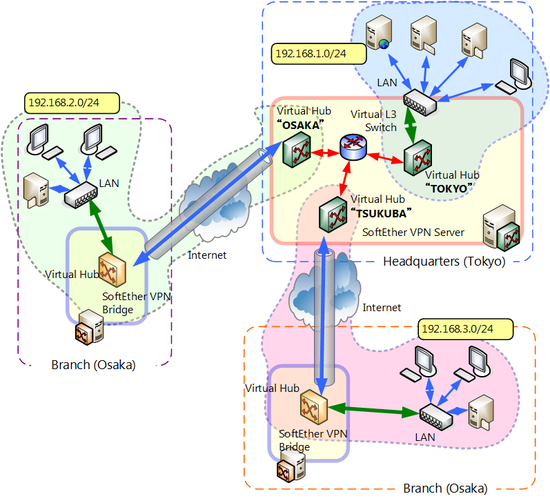
\includegraphics[scale=0.45]{img/softether_l3_lan_to_lan}
        \label{fig:softether_l3_lan_to_lan}
        \caption[Configurazione LAN-to-LAN con SoftEther al layer 3]{Configurazione LAN-to-LAN con SoftEther al layer 3.}
      \end{figure}
    \end{enumerate}
  \end{itemize}
\end{itemize}
SoftEther possiede alcune caratteristiche molto interessanti, oltre a quelle già citate:
\begin{description}
  \item[\textbf{VPN over ICMP} e \textbf{VPN over DNS}]Due opportunità non completamente stabili (il sito ufficiale stesso
  riporta che a volte si verificano degli errori) per il quale si incapsula il traffico in pacchetti ICMP
  o DNS per bypassare anche i firewall più stringenti. Occorre valutare \textit{quanto}
  siano stringenti tali firewall, perché anche queste soluzioni potrebbero non essere
  praticabili (ad esempio se si usa un server DNS interno e sul firewall si configura l'abilitazione
  al protocollo DNS solo se proveniente da tale server).
  \item[\textbf{NAT Traversal}]Se il server si trova dietro ad un NAT, è comunque possibile connettersi poiché
  esso si occupa di fare continue connessioni verso l'esterno in modo che, quando un client tenta di connettersi
  il NAT lascia passare la connessione, similmente a quanto fatto da Skype.
  \item[\textbf{Dyamic DNS}]Non occorre che si possieda un indirizzo IP statico per identificare il server.
  Gratuitamente SoftEther registra un nuovo nome DNS per ciascun server che viene installato, ed aggiorna
  automaticamente tale nome sulla base degli assegnamenti degli ISP (verificando quale sia l'IP
  del server che si connette all'infrastruttura SoftEther).
  \item[\textbf{SecureNAT}]Si tratta di una tecnologia sviluppata appositamente per SoftEther ed è integrata
  nel server, e consiste di un DHCP+NAT. Va notato che questa funzione non richiede privilegi particolari,
  poiché è eseguita in user-space (in Windows, mentre per Linux occorrerebbe verificare se non siano
  richiesti i privilegi di root).
  Per ciascun \textit{Virtual Hub} è possibile abilitare questa funzione, ciò fa sì che si crei
  una nuova interfaccia di rete virtuale connessa al \textit{Virtual Hub}
  come se fosse un altro computer collegato in VPN, ed infatti, per gli altri host, la scheda virtuale appare proprio
  come un altro computer. Può essere usato per vari scopi:
  \begin{itemize}
    \item Network Gateway: \textit{SecureNAT} può essere usato come alternativa al \textit{Local Bridge} per
    connettere un \textit{Virtual Hub} alla rete fisica. Si usa una nuova interfaccia virtuale che viene connessa al \textit{Virtual Hub}.
    \item DHCP Server: è possibile scegliere di abilitare solo la funzione di DHCP Server in \textit{SecureNAT}, pertanto
    tale server assegnerà gli indirizzi IP agli alle interfacce dei client connesse al \textit{Virtual Hub} a cui
    l'interfaccia \textit{SecureNAT} è collegata.
    \item Remote Access. Questa è in assoluto la caratteristica più interessante, le cui potenzialità andrebbero studiate
    nel dettaglio. Normalmente, quando ci si vuole connettere ad una rete da remoto è
    necessario installare su in essa \textit{VPN Server}, e di conseguenza connettersi da un client. Usando \textit{SecureNAT}
    è invece possibile invertire questo paradigma. La figura \ref{fig:securenat} illustra la topologia che si realizza.\\
    \begin{figure}
      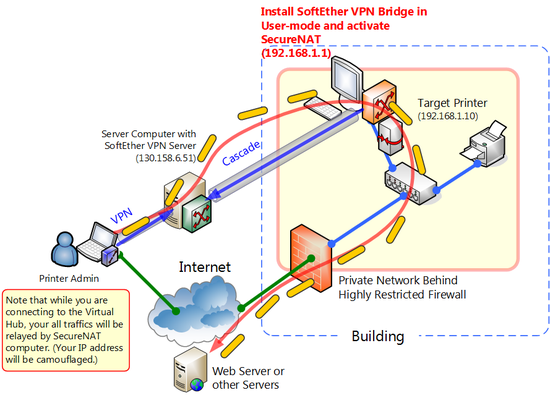
\includegraphics[scale=0.55]{img/securenat}
      \label{fig:securenat}
      \caption[La topologia realizzata con \textit{SecureNAT}]{La topologia realizzata con \textit{SecureNAT}.}
    \end{figure}
    Senza scendere troppo nei dettagli, si illustrano gli step necessari. Per \textit{rete remota} si intende la rete a cui
    ci si vuole connettere, per \textit{rete principale} si intende la rete da cui la connessione parte, ovvero
    la rete da cui l'utente fisicamente si collega.
    \begin{enumerate}
      \item Sulla rete principale si crea un server con \textit{Virtual Hub}
      \item su un host della \textit{rete remota} si installa e si esegue il \textit{VPN Bridge}
      \item si abilita la funzione di \textit{SecureNAT} sul \textit{VPN Bridge} (può essere fatto da remoto
      usando la GUI oppure la command line utility)
      \item si configura il server della rete principale per creare una nuova connessione verso il \textit{VPN Bridge}.\\
      Ciò che accade è che si è stabilita una \textit{cascaded connection} tra il bridge ed il server (il \textit{Virtual Hub}
      del server).
      \item Per utilizzare davvero questo funzionalità l'utente usa un client VPN e si connette al server. La NIC
      del client sarà configurata dal DHCP Server di \textit{SecureNAT} integrato nel bridge,
      ed il bridge stesso sarà il suo default gateway. Tutto il traffico del client andrà verso il bridge, e dal bridge poi
      uscirà su internet (usando l'IP pubblico del NAT dietro a cui c'è il bridge). Grazie a ciò che SoftEther offre,
      non è necessaria alcuna configurazione nella rete remota (se non l'installazone del \textit{VPN Bridge}).
    \end{enumerate}
  \end{itemize}
  \item[\textbf{Performance}]Secondo dei test eseguiti nel 2012 SoftEther \textit{VPN Server} è più veloce (maggiore throughput) di tutte le
  altre alternative. Il grafico in figura \ref{fig:softether-performance} mostra il risultato dei test. Si tenga comunque
  conto che sono benchamrk vecchi di 5 anni.
\end{description}
\begin{figure}
  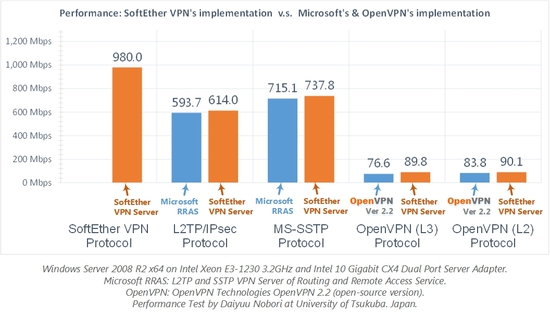
\includegraphics[scale=0.4]{img/softether_perf}
  \caption[Comparazione performance delle diverse tecnologie VPN]{Comparazione performance delle diverse tecnologie VPN (2012).}
  \label{fig:softether-performance}
\end{figure}

\subsection{SoftEther e MoonCloud}
Dopo aver analizzato SoftEther ora si vedono quali sono le possibili configurazioni per un suo uso in MoonCloud.
Si è valutata come migliore soluzione quella basata su incapsulamento in HTTPS di L3.
La prima distinzione sta nel dove posizionare il server.
\begin{description}
  \item[\textbf{Nel cloud}]Installare il server nella rete MoonCloud pone un problematica
  non così banale, cioè la necessità (non mandatoria ma caldamente consigliata) di
  disporre di una scheda di rete da poter configurare in modalità promiscua, ovviamente
  a livello di VM. E' possibile che dei cloud provider non consentano questo.
  Nella rete target si porterebbe un'appliance con \textit{VPN Bridge}.
  \item[\textbf{Nella rete target}]In questa configurazione, se l'implementazione
  di NAT Traversal di SoftEther lo consente, sarebbe possibile per i client raggiungere
  il server nella rete target anche se dietro ad un NAT. Occorrerebbe poi valutare utilizzare
  un unico client in MoonCloud (\textit{RSSC}) oppure diversi (\textit{RSMC}); ovviamente
  per \textit{unico client} si intende un \textit{unico} client per ciascuna rete.
\end{description}
In ogni caso, nemmeno SoftEther poteva eliminare la necessità di configurare rotte
nella rete target, se non con l'utilizzo del già citato \textit{NAT al contrario}.

Oltre a queste soluzioni classiche, si sarebbe potuto sfruttare anche \textit{Secure NAT}.
Si tratta di una modalità interessante, che avrebbe richiesto uno studio approfondito
per capire come potesse davvero aiutare il nostro use case.
In questo caso:
  \begin{itemize}
    \item l'appliance è costituita dal \textit{VPN Bridge};
    \item in MoonCloud si installa il server;
    \item i container sono client VPN che si connettono al server.
  \end{itemize}


\subsection{Conclusioni}
Per SoftEther, in forza del NAT Traversal, si è consigliato di realizzare una topologia
\textit{Remote Server}, eventualmente combinabile con il Dynamic DNS fornito
da SoftEther o con uno gestito da MoonCloud.
Un ulteriore ed importante vantaggio è che SoftEther utilizza HTTPS. Per tutte queste
ragioni SoftEther è stata inizialmente preferita rispetto ad OpenVPN.
